\section{Mechanische Konstruktion und Fertigung}
Die mechanische Basis des Systems bildet eine Multiplexplatte, die als tragende Struktur dient.  
Auf dieser Grundplatte werden die LED-Streifen montiert und die Frontabdeckung verschraubt.  
Der Mikrocontroller wird auf der Rückseite der Platte befestigt.  
Für die Darstellung der Wortmatrix werden Bauteile konstruiert und mittels \gls{3ddruck} aus schwarzem \gls{pla} hergestellt.
Ein Beispiel dafür ist in Abb.~\ref{fig:3DDruckbeispiel} dargestellt.
\begin{figure}[H]
	\centering
	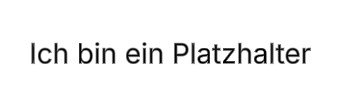
\includegraphics[width=0.3\linewidth]{inhalt/bilder/Platzhalter.jpg}
	\caption{Fertiggestellter Druck des Frontplattenbauteil Nr. 11 auf dem 3D-Drucker Kobra S1 der Marke Anycubic.}
	\label{fig:3DDruckbeispiel}
\end{figure}
Die gedruckten Bauteile bilden die Frontplatte sowie die Einhausung der LEDs.  
Die Konstruktion basiert auf einer modularen Struktur aus insgesamt 16 Einzelteilen (vgl. Abb.~\ref{fig:Frontplatte}), welche miteinander verschraubt werden.  
Dadurch entsteht eine zusammenhängende Frontabdeckung mit den Abmessungen H x B x T.    
\begin{figure}[H]
	\centering
	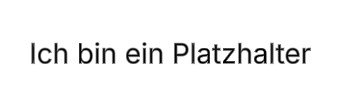
\includegraphics[width=0.3\linewidth]{inhalt/bilder/Platzhalter.jpg}
	\caption{}
	\label{fig:}
\end{figure}
Die Bauteile werden in drei Grundtypen unterteilt.  
Es existieren Mittelstücke, Eckstücke und Seitenstücke (vgl. Abb.~\ref{fig:Frontplatte}).  
Alle Bauteile folgen demselben konstruktiven Prinzip, unterscheiden sich jedoch in der jeweiligen Buchstabenbelegung oder Symbolik.  

Die Hauptanzeige, die aus 16 mal 16 Buchstaben besteht, dient der Darstellung der Uhrzeit, der Außentemperatur und des Wetters.  
Zusätzlich werden Symbole für die Zusatzfunktionen integriert, welche links, rechts, ober- und unterhalb der Buchstabenmatrix angeordnet sind (vgl. Abb.~\ref{fig:Frontplatte}).  
Diese umfassen die Anzeige von Raumfeuchtigkeit, Innenraumtemperatur, Mondphase und Tageszeit (vgl. Abb.~\ref{fig:ZusatzfunktionenaufderUhr}).  
\begin{figure}[H]
    \centering
    \begin{subfigure}[t]{0.48\textwidth}
        \centering
        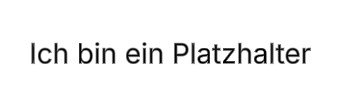
\includegraphics[width=\linewidth]{inhalt/bilder/Platzhalter.jpg}
        \caption{links oben}
        \label{fig:Raumfeuchtigkeit}
    \end{subfigure}
    \hfill
    \begin{subfigure}[t]{0.48\textwidth}
        \centering
        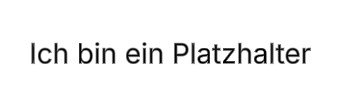
\includegraphics[width=\linewidth]{inhalt/bilder/Platzhalter.jpg}
        \caption{rechts oben}
        \label{fig:Innenraumtemperatur}
    \end{subfigure}
    \vspace{0.8em}
    \begin{subfigure}[t]{0.48\textwidth}
        \centering
        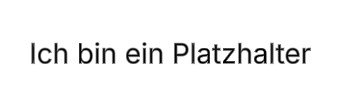
\includegraphics[width=\linewidth]{inhalt/bilder/Platzhalter.jpg}
        \caption{links unten}
        \label{fig:Mondphase}
    \end{subfigure}
    \hfill
    \begin{subfigure}[t]{0.48\textwidth}
        \centering
        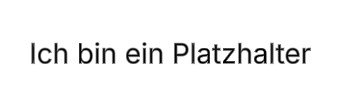
\includegraphics[width=\linewidth]{inhalt/bilder/Platzhalter.jpg}
        \caption{rechts unten}
        \label{fig:Tageszeit}
    \end{subfigure}
    \caption{Darstellung der vier Zusatzfunktionen die die Wortuhr neben der Uhrzeit, der Außentemperatur und dem Wetter anzeigen.}
    \label{fig:ZusatzfunktionenaufderUhr}
\end{figure}
Die Sekundenanzeig ist am Ausenrand der Frontplatte mit 60 Schlitzen realisiert (vgl. Abb.~\ref{fig:Frontplatte}).

Die Verbindung zur Grundplatte erfolgt über die Eckstücke.  
Hierzu werden Gewindeeinsätze, sogenannte Heatinsert, eingesetzt, welche in das 3D-gedruckte Material integriert werden (vgl. Abb.~\ref{fig:Heatinserts}).
Hierzu werden die Heatinserts z.B. mit einem Lötkolben mit geeigneter Spitze erhitzt und dann eingepresst.
\begin{figure}[H]
	\centering
	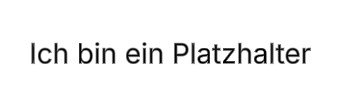
\includegraphics[width=0.3\linewidth]{inhalt/bilder/Platzhalter.jpg}
	\caption{}
	\label{fig:}
\end{figure}  
Die Befestigung erfolgt anschließend mit M4x20-Schrauben.  
Die Verbindung der einzelnen Frontbauteile untereinander erfolgt über Durchgangsbohrungen.  
Hierbei werden M3x12-Schrauben in Kombination mit Muttern und Unterlegscheiben verwendet.  

Zur Verbesserung der Lichtverteilung werden für jeden Buchstaben sowie jedes Symbol separate Diffusorplättchen eingesetzt.  
Diese werden ebenfalls im 3D-Druckverfahren aus weißem \gls{pla} hergestellt und dann eingeklebt.  
Die Plättchen besitzen eine Dicke von 0.4 mm, was einer Layerhöhe von 2 entspricht. 
Das bedeutet, der Drucker druckt nur 2 Schichten \gls{pla} übereinander.  
Die optimale Dicke wurde empirisch ermittelt, um eine gleichmäßige Lichtstreuung ohne signifikante Helligkeitsverluste zu erreichen.  
Zusätzlich wurden Bauteile als Abstandshalter zur Wand und gleichzeitig als Aufhängungspunkte konstruiert.   
Weiterhin wurde eine Montageplatte für den Mikrocontroller entwickelt, welche an der Rückseite der Multiplexplatte montiert ist.  
Dadurch bleibt die USB-C-Schnittstelle des Mikrocontroller auch im montierten Zustand erreichbar. 
\begin{figure}[H]
    \centering
    \begin{subfigure}[t]{0.32\textwidth}
        \centering
        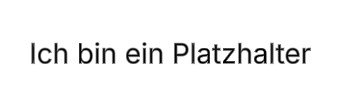
\includegraphics[width=\linewidth]{inhalt/bilder/Platzhalter.jpg}
        \caption{3D gedrucktes Diffusorplättchen mit einer dicke von 0,4 mm.}
        \label{fig:Diffusor}
    \end{subfigure}
    \hfill
    \begin{subfigure}[t]{0.32\textwidth}
        \centering
        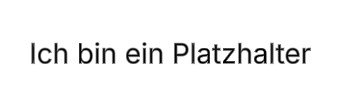
\includegraphics[width=\linewidth]{inhalt/bilder/Platzhalter.jpg}
        \caption{3D gedruckte Abstandshalter und Befestigungspunkte der Wortuhr.}
        \label{fig:Abstandshalter}
    \end{subfigure}
    \hfill
    \begin{subfigure}[t]{0.32\textwidth}
        \centering
        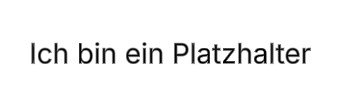
\includegraphics[width=\linewidth]{inhalt/bilder/Platzhalter.jpg}
        \caption{3D gedruckte Montageplatte für den ESP32-C6, welche an der Rückseite montiert wird.}
        \label{fig:MontageplatteESP}
    \end{subfigure}
\end{figure}